% !TEX encoding = UTF-8 Unicode
\documentclass[a4paper]{article}

\usepackage{color}
\usepackage{url}
\usepackage[T2A]{fontenc} % enable Cyrillic fonts
\usepackage[utf8]{inputenc} % make weird characters work

\usepackage{graphicx}
\usepackage{xcolor}

\usepackage[english,serbian]{babel}
%\usepackage[english,serbianc]{babel} %ukljuciti babel sa ovim opcijama, umesto gornjim, ukoliko se koristi cirilica

\usepackage[unicode]{hyperref}
\hypersetup{colorlinks,citecolor=green,filecolor=green,linkcolor=blue,urlcolor=blue}

\usepackage{listings}
\renewcommand{\lstlistingname}{Kod} %da ne bi pisalo Listing 1

%\newtheorem{primer}{Пример}[section] %ćirilični primer
\newtheorem{primer}{Primer}[section]

\definecolor{mygreen}{rgb}{0,0.6,0}
\definecolor{mygray}{rgb}{0.5,0.5,0.5}
\definecolor{mymauve}{rgb}{0.58,0,0.82}

\lstset{ 
  backgroundcolor=\color{white},   % choose the background color; you must add \usepackage{color} or \usepackage{xcolor}; should come as last argument
  basicstyle=\scriptsize\ttfamily,        % the size of the fonts that are used for the code
  breakatwhitespace=false,         % sets if automatic breaks should only happen at whitespace
  breaklines=true,                 % sets automatic line breaking
  captionpos=b,                    % sets the caption-position to bottom
  commentstyle=\color{mygreen},    % comment style
  deletekeywords={...},            % if you want to delete keywords from the given language
  escapeinside={\%*}{*)},          % if you want to add LaTeX within your code
  extendedchars=true,              % lets you use non-ASCII characters; for 8-bits encodings only, does not work with UTF-8
  firstnumber=1,                % start line enumeration with line 1
  frame=single,	                   % adds a frame around the code
  keepspaces=true,                 % keeps spaces in text, useful for keeping indentation of code (possibly needs columns=flexible)
  keywordstyle=\color{blue},       % keyword style
  language=Python,                 % the language of the code
  morekeywords={*,...},            % if you want to add more keywords to the set
  numbers=left,                    % where to put the line-numbers; possible values are (none, left, right)
  numbersep=5pt,                   % how far the line-numbers are from the code
  numberstyle=\tiny\color{mygray}, % the style that is used for the line-numbers
  rulecolor=\color{black},         % if not set, the frame-color may be changed on line-breaks within not-black text (e.g. comments (green here))
  showspaces=false,                % show spaces everywhere adding particular underscores; it overrides 'showstringspaces'
  showstringspaces=false,          % underline spaces within strings only
  showtabs=false,                  % show tabs within strings adding particular underscores
  stepnumber=2,                    % the step between two line-numbers. If it's 1, each line will be numbered
  stringstyle=\color{mymauve},     % string literal style
  tabsize=2,	                   % sets default tabsize to 2 spaces
  title=\lstname                   % show the filename of files included with \lstinputlisting; also try caption instead of title
}

\begin{document}

\title{Profajleri i njihova vizualizacija u jeziku Python\\ \small{Seminarski rad u okviru kursa\\Metodologija stručnog i naučnog rada\\ Matematički fakultet}}

\author{
Anđelka Milovanović, David Popov \\
Jelisaveta Smiljanić, Petar Zečević \\
mi15145@alas.matf.bg.ac.rs, mi16102@alas.matf.bg.ac.rs \\
mi16138@alas.matf.bg.ac.rs, mi16169@alas.matf.bg.ac.rs 
}

%\date{9.~april 2015.}

\maketitle

\abstract{
Tema ovog seminarskog rada je vezana za profajlere u programskom jeziku {\em Python}. Osnovni cilj rada je da se čitaoci upoznaju sa različitim alatima za profajliranje, njihovim mogućnostima i praktičnom primenom kroz primere u jeziku Python. Takođe, jedan od ciljeva je da se čitalac ubedi zašto je korisno koristiti profajlere i kako oni mogu značajno pomoći u analiziranju napisanog koda i njegovog efikasnijeg izvršavanja.}

\setcounter{tocdepth}{2} 
\tableofcontents

\newpage
\section{Uvod}
\label{sec:uvod}

Optimizacija koda je značajan deo razvoja svih ozbiljnijih i kompleksnijih softvera \cite{opt}. Postavlja se pitanje koje delove koda treba razmatrati za ovakve promene, kada kod treba razmatrati i da li ga uopšte treba razmatrati. Kod softvera složenijeg dizajna i arhitekture, teško je intuitivno zaključiti šta treba optimizovati. Upravo sa ciljem jednostavnijeg, temeljnijeg i bržeg procesa ispitivanja kodova nastali su \textbf{profajleri} \cite{profiling}.

U nastavku ovog rada biće reči o profajlerima generalno, kao i o njihovoj podeli na  determinitstičke i statističke. Zatim se prelazi na profajliranje u jeziku Python, gde se govori o profajlerima profile, cProfile i hotshot. Konačno, uvešće se priča o alatima za vizualizaciju, gde će biti opisan i pokazan rad nekih od najpoznatijih alata: Py-Spy, SnakeViz, Pycallgraph, Gprof2dot i Vprof.

Svi profajleri i alati za vizualizaciju su testirani na kodu \ref{lst:test_code} datom u dodatku rada. Kod se sastoji od funkcija koje na različite načine računaju n-ti Fibonačijev broj \cite{fib}.

\section{Šta je profajliranje?}	
\label{sec:profajliranje}

Profajliranje je proces koji značajno pomaže da se detektuju delovi koda koji mogu da učine program optimalnim. Optimizacijom koda možemo smanjiti vreme izvršavanja, memoriju koja se koristi ili detektovati mrežno opterećenje kojim se troši vreme na dohvatanje informacija \cite{mit}. Postoje različiti načini kako možemo profajlirati kod. Za vremensko profajliranje postoji jednostavna komanda u konzoli {\em time} kojom možemo dobiti kratak izveštaj izvršavanja celog programa (videti sliku \ref{fig:time_shell}) ili modul {\em time} u Python-u kojim možemo meriti vreme unutar koda (videti primer \ref{lst:kod_time}). Kako su ovi načini ponekad nedovoljni ili naporni za implementaciju kod programa složenije strukture, programeri su osmislili alate koji služe za automatsko profajliranje koda i detektovanje kritičnih delova \cite{vanderplas2016python}. Ti alati se nazivaju profajleri.

Profajliranje se deli na \textbf{determinističko} (eng. tracing) i na \textbf{statističko} (eng. sampling). \textbf{Determinističko} profajliranje se izvršava zajedno sa kodom i profajleri beleže svako pokretanje i svako završavanje funkcije u programu. Loša strana ovakvog načina profajliranja je što je skupo, jer ugrožava performanse programa time što mora da prati stanje svih funkcija. To može dovesti do nerealne predstave o tome koliko je koja funkcija na primer vremenski zaista zahtevna, jer profajliranje takođe oduzima neko vreme \cite{deterministic}. \textbf{Statističko} profajliranje (uzoračko) se vrši uzorkovanjem vrednosti u IP (eng. Instruction Pointer) registru dok program radi. Uzorci se povezuju sa konkretnim funkcijama i potprogramima, a zatim se vrši statistička analiza da bi se odredilo koji se delovi koda najduže izvršavaju \cite{StatProf1}. Ni ovakvim profajliranjem se ne dobijaju tačni rezultati, jer se program ne posmatra u svakom trenutku izvršavanja. Stanje se posmatra samo u tim trenucima koji se uzorkuju, što je ujedno i najveća mana statističkog profajliranja. Prednost u odnosu na determinističko profajliranje je manja memorijska zahtevnost da bi se podaci skladištili, kao i manje vremena potrebnog da se profajliranje izvrši iz razloga što se program posmatra periodično \cite{StatProf2}.

Pored podele na determinističko i statističko, profajliranje se može razlikovati i prema tome da li meri vremensko ili memorijsko opterećenje \cite{lanaro2013python}. U daljem tekstu biće dati primeri takvih profajliranja kroz programski jezik Python. 

\section{Načini profajliranja u jeziku Python}	
\label{sec:profajleri_u_pythonu}
Osnovni vid vremenskog profajliranja u jeziku Python se može prikazati korišćenjem modula {\em time}. Pokretanjem koda \ref{lst:kod_time} koji se nalazi u sekciji \ref{sec:dodatak}, kao izlaz iz programa dobija se uvek neka vrednost veća od postavljene vrednosti za promenljivu {\em n}. Na primer, izlaz može biti nešto poput:

\begin{quote}
    {\em Ukupno je proteklo 5.002248048782349 sekundi.}
\end{quote}
Razlog zašto je izmereno vreme veće od očekivanog je to što je ovo vreme celokupnog izvršavanja programa od njegovog pokretanja do kraja. To vreme nije isto kao vreme koje naš program provodi koristeći procesorsku jedinicu, jer u tom trenutku pokretanja našeg programa ima još aktivnih procesa koji se izvršavaju na procesoru. Dakle, postoje tri različite vrste vremena koja se mere: stvarno (eng. real or total), korisničko (eng. user) i sistemsko (eng. system). Korisničko meri kumulativno vreme provedeno na procesoru prilikom izračunavanja, dok sistemsko meri vreme potrošeno na memorijske alokacije \cite{lanaro2013python}. Dodavanjem komande {\em time} u konzoli UNIX sistema, pre pokretanja neke druge komande, može se dobiti kratak izveštaj za ova tri vremena (za svaki operativni sistem je drugačije, a primer na macOS Catalina, u zsh terminalu nad kodom \ref{lst:kod_time} prikazan je na slici \ref{fig:time_shell}). Pokretanjem koda \ref{lbl:cmodule_test} na četiri različita računara svakog od autora (konfiguracije računara videti u tabeli \ref{table:performance}), dobijena su vremena i predstavljena kroz barplot na slici \ref{fig:custom_time}.

\begin{figure}[h!]
\begin{center}
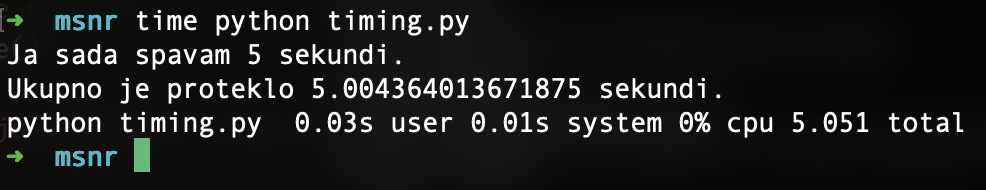
\includegraphics[scale=0.6]{MVJ_02_ProfajleriZaPython_ZecevicSmiljanicMilovanovicPopov/time_python_shell.png}
\end{center}
\caption{UNIX komanda {\em time}.}
\label{fig:time_shell}
\end{figure}

\begin{figure}[h!]
\begin{center}
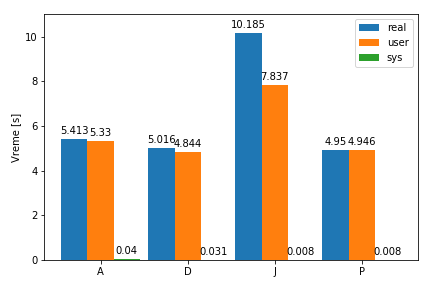
\includegraphics[scale=0.7]{MVJ_02_ProfajleriZaPython_ZecevicSmiljanicMilovanovicPopov/barplot.png}
\end{center}
\caption{Vremena potrebna za izvršavanje istog koda na 4 računara.}
\label{fig:custom_time}
\end{figure}


Drugi način da se celine programa u jeziku Python vremenski proprate je korišćenjem modula {\em timeit}. Modul meri vreme potrebno da se neki deo koda izvrši tako što ga pokreće u petlji n puta. Ovakav proces može da se ponavlja r puta, nakon čega uzima najbolju dobijenu vrednost kao konačnu. Zbog načina na koji radi, korisno ga je koristiti samo za \textbf{precizno} merenje malih delova koda \cite{lanaro2013python}, zbog čega se neće detaljnije razmatrati.

Preporuka je da se profajliranje, kao i sve optimizacije koda, rade tek na samom kraju projekta, jer preuranjeno optimizovanje može biti koren svih nevolja \cite{knuth}.
Nakon što se izmeri vreme izvršavanja celog programa, mogu se identifikovati celine koje bi mogle potencijalno da se unaprede i ubrzaju. U jeziku Python za to postoje 3 ugrađena modula iz standardne biblioteke: 
\begin{itemize}
  \item profile
  \item hotshot
  \item cProfile
\end{itemize}
Ovi ugrađeni moduli obezbeđuju determinističko profajliranje. Statističko ugrađeno profajliranje ne postoji, ali postoje biblioteke za rad sa njim.

Modul {\em profile} je pisan u čistom Python-u i njegovo izvršavanje može da bude skupo za performanse. Modul {\em hotshot} je znatno brži, pisan je u jeziku C, ali se ne koristi toliko često i nije podržan u Python 3. Najkorišćeniji modul za profajliranje je {\em cProfile}, pisan je u C jeziku i njegove funkcionalnosti su slične prvom modulu, ali je znatno brži \cite{cProfile}. U narednoj celini detaljnije će biti obrađen ovaj modul, jer je najkorišćeniji i najviše alata se oslanja na njega.

\subsection{Moduli cProfile i pstats}
Da bi se dobio izveštaj profajliranja kroz {\em cProfile} modul, potrebno je pokrenuti komandu \cite{cProfile}: 
\begin{lstlisting}[language=bash, belowskip=-\baselineskip, frame=single]
  $ python -m cProfile test_kod.py
\end{lstlisting}
Test kod predstavlja funkcije definisane u primeru \ref{lst:test_code}, sa izmenom:
\begin{lstlisting}[caption={Dodatak za testiranje {\em cProfile}.},frame=single, 
label=lbl:cmodule_test]
number = 20
print('Input number is: ' + str(number))
for i in range(0, 1000):
    for_fib(number)
    recur_fib(number)
    tail_recur_fib(number)
    functional_fib(number)
\end{lstlisting}
\begin{figure}[h!]
\begin{center}
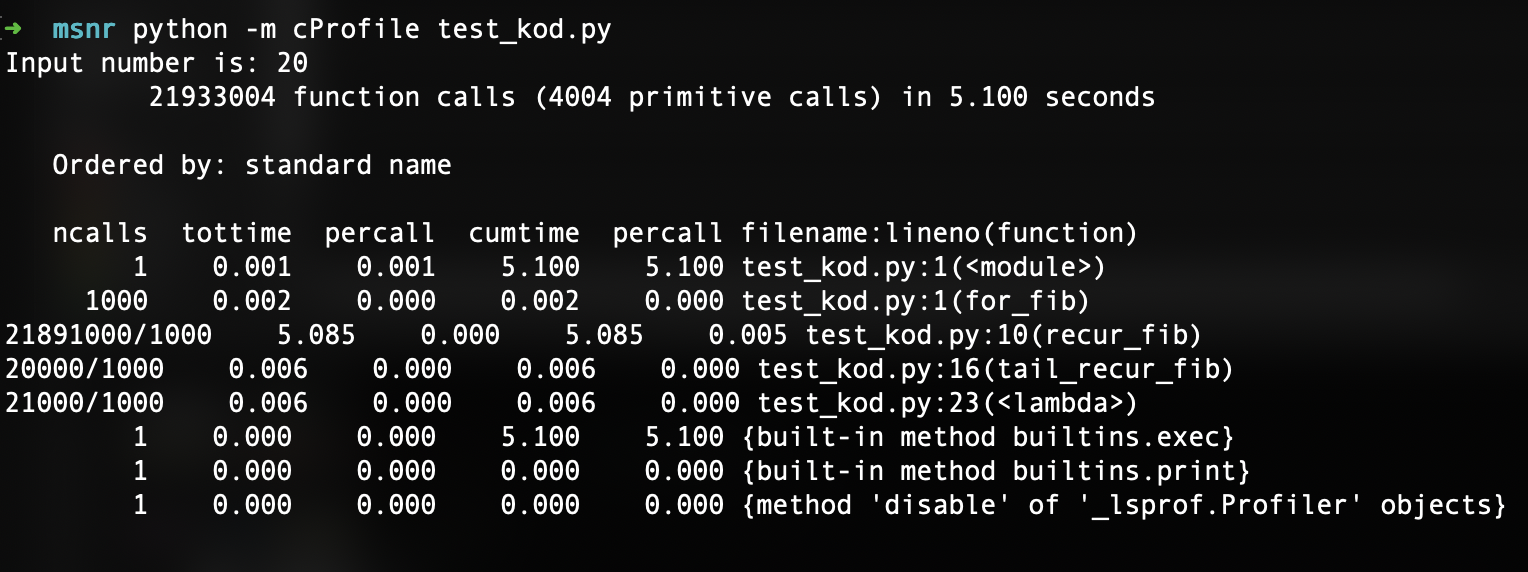
\includegraphics[scale=0.4]{MVJ_02_ProfajleriZaPython_ZecevicSmiljanicMilovanovicPopov/cProfile_without_import.png}
\end{center}
\caption{Primer izveštaja iz cProfile modula.}
\label{fig:cProfile_no_import}
\end{figure} 

Ono što se može videti iz izveštaja \ref{fig:cProfile_no_import} je koliko funkcijskih poziva je ispratio cProfile i koliko njih su primitivni pozivi. U ovom slučaju samo 4004 poziva su bila primitivna, dok su ostali pozvani rekurzijom. Sve je sortirano prema poslednjoj koloni (što može da se modifikuje), a u tabeli \ref{tab:cProfile_args} su objašnjeni preostali argumenti \cite{cProfile}. Izveštaj koji napravi cProfile može da se napravi unutar programa i sačuva u obliku fajla, a zatim obradi i formatira putem klase {\em Stats} modula {\em pstats}. Uključivanje zaglavlja, startovanje funkcije i čuvanje izveštaja se postiže komandama: \newpage
\begin{lstlisting}[caption={Primer čuvanja izveštaja u fajl.},frame=single, label=lbl:cProfile_report]
import cProfile
# ... ovde se nalaze funkcije
cProfile.run('test_function()', './izvestaj')
\end{lstlisting}
Modul {\em pstats} sadrži veliki broj mogućnosti za filtriranje dobijenih informacija iz izveštaja. Na primer, ukoliko je cilj da se razume koji algoritam oduzima najviše vremena, sortiranje izveštaja treba da se vrši po koloni {\em cumulative}, nakon čega se komandom {\em print\_stats(5)} može izdvojiti 5 vremenski najzahtevnijih poziva. Takođe, moguće je kombinovati module {\em cProfile} i {\em pstats} i jedan takav primer je prikazan u kodu \ref{lst:cprofile_pstats}. Klasa {\em Stats} može da napravi instance od izveštaja koji su u fajlovima ili direktno od {\em Profile} klase. Nad njima se mogu pozivati metode poput: {\em strip\_dirs, add, dump\_stats, sort\_stats, print\_stats}, o kojima se više može videti na \cite{cProfile}.
\vspace{-5pt}
\begin{table}[h!]
\begin{center}
\caption{Argumenti iz cProfile izveštaja i njihovi opisi.}
\begin{tabular}{|l|l|} \hline
\textbf{ARGUMENT} & \textbf{OPIS} \\ \hline
ncalls & broj poziva\\ \hline
tottime & ukupno vreme funkcije\\ \hline
percall & tottime/ncalls\\ \hline 
cumtime & ukupno vreme funkcije i svih podfunkcija\\ \hline
percall & cumtime/primitive calls\\ \hline
filename:lineno(function) & podaci o funkciji \\ \hline
\end{tabular}
\label{tab:cProfile_args}
\end{center}
\end{table}
\vspace{-20pt}
\section{Alati za vizualizaciju profajliranja}
Statistika koja se dobije profajliranjem postaje nečitljivija što je program kompleksniji. Da bi dobijeni rezultat bio što pregledniji, razvijeni su razni alati za vizualizaciju profajliranja. U ovom poglavlju dati su neki alati u jeziku Python (više alata može se naći na \cite{VizList}). Kao i do sada, svi alati se testiraju na kodu \ref{lst:test_code} koji se nalazi u dodatku.
    
\subsection{Py-Spy}
\label{profajler_3}
\textbf{Py-Spy} je statistički profajler za jezik Python koji omogućava vizualizaciju informacija o izvršavanju programa tokom njegovog rada. Napisan je u programskom jeziku Rust. Može da se koristi na operativnim sistemima Linux, OSX i Windows, a podržava verzije 2.3-2.7 i 3.3-3.7 Python-a \cite{PySpy1}. Instalira se pomoću naredne komande:
\begin{lstlisting}[language=bash, belowskip=-\baselineskip]
  $ pip install py-spy
\end{lstlisting}
Py-spy se pokreće preko komandne linije tako što mu se da PID (eng. process identificator) procesa:
\begin{lstlisting}[language=bash, belowskip=-\baselineskip]
  $ py-spy --pid 12345
\end{lstlisting}
ili ime programa koji želimo da profajliramo:
\begin{lstlisting}[language=bash, belowskip=-\baselineskip]
  $ py-spy -- python myprogram.py
\end{lstlisting}
Detaljna instalacija i pokretanje mogu se naći na \cite{PySpy1}.
\subsubsection{Karakteristike alata}
Py-Spy je uzorački profajler, što znači da program mora da bude u toku izvršavanja kada se alat pokrene. Dakle, on omogućava profajliranje programa koji moraju neprestano da rade. Većina profajlera zahteva da se kod modifikuje na neki način, dok Py-Spy ne samo da ne zahteva modifikacije koda, već se izvršava u zasebnom programu čime smanjuje vreme izvršavanja i ne ometa rad programa ni na jedan način \cite{PySpy2}. Glavna mana Py-Spy profajlera je ujedno i glavna mana statističkog profajliranja: procena umesto tačnog rešenja usled uzorkovanja podataka \cite{StatProf2}. 
\subsubsection{Primer primene}
Pokretanjem alata Py-Spy dobija se slika programa sa trajanjem svih funkcija u njemu. Pokrenut je referentni program ali u beskonačnoj petlji, da bi Py-Spy mogao da uzorkuje u vreme izvršavanja programa. Rezultat pokretanja prikazan je na slici \ref{fig:ps_viz}. Što funkcija traje duže, linija kojom je ona predstavljena je duža. Takođe, može se videti redosled poziva funkcija. 
\begin{figure}[h!]
\begin{center}
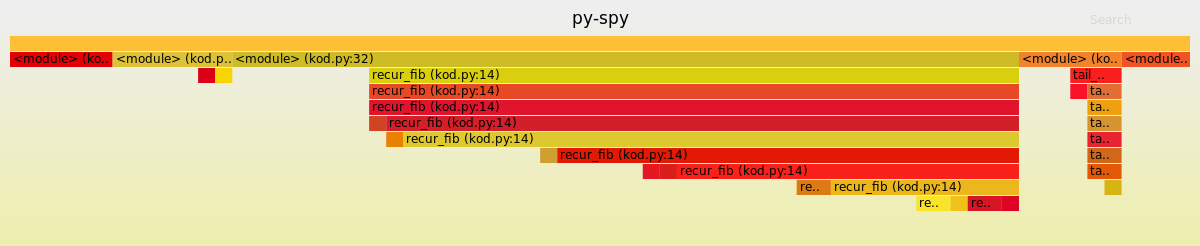
\includegraphics[scale=0.26]{MVJ_02_ProfajleriZaPython_ZecevicSmiljanicMilovanovicPopov/ps.png}
\end{center}
\caption{Py-Spy vizualizacija.}
\label{fig:ps_viz}
\end{figure}

\subsection{SnakeViz} 
\label{profajler_2}
\textbf{SnakeViz} je alat za vizualizaciju statistike profajliranja koji je generisan od strane {\em cProfile} modula i predstavlja alternativu {\em pstats} modulu. Inspirisan je RunSnakeRun alatom. Snakeviz podržava verzije interpretera Python 2.7 i Python 3 \cite{SnakeViz1}. Fajl koji se generiše je u formatu .profile. Alat SnakeViz se instalira pomoću naredne komande:
\begin{lstlisting}[language=bash, belowskip=-\baselineskip]
  $ pip install snakeviz --user
\end{lstlisting}
Kada se pokreće Python kod, potrebno je navesti ime fajla u formatu .profile:
\begin{lstlisting}[language=bash, belowskip=-\baselineskip]
  $ python -m cProfile -o test.profile test.py
\end{lstlisting}
Zatim je potrebno izvršiti sledeću komandu da bi se dobila vizualizacija u obliku .html fajla:
\begin{lstlisting}[language=bash, belowskip=-\baselineskip]
  $ snakeviz test.profile
\end{lstlisting}
Detaljnije informacije o instalaciji i pokretanju alata mogu se naći na \cite{SnakeViz1}.
\subsubsection{Karakteristike alata}
 SnakeViz nije u mogućnosti da podrži velike profile zbog poteškoća reprezentovanja ogromnih stabala pomoću JSON niski. Za sada se smatra da SnakeViz može da podrži stabla sa manje od nekoliko hiljada čvorova. Međutim, iako ne uspe da napravi vizualizaciju i dalje će se dobiti potpuna tabela statistika. To znači da neuspeh vizualizacije SnakeViz alata ne utiče na samo izvršavanje profajliranja \cite{SnakeViz2}. Alat SnakeViz omogućava izbor kriterijuma po kom se podaci u tabeli sortiraju.
\subsubsection{Primer primene}
Pokretanjem SnakeViz alata otvara se .html fajl u veb pretraživaču. Vizualizacija se može predstaviti u {\em Iciclie} i {\em Sunburst} formatu. Na slici \ref{fig:snake_viz_1} je dat primer koda nad kojim se testiraju vizualizacije.
\begin{figure}[h!]
\begin{center}
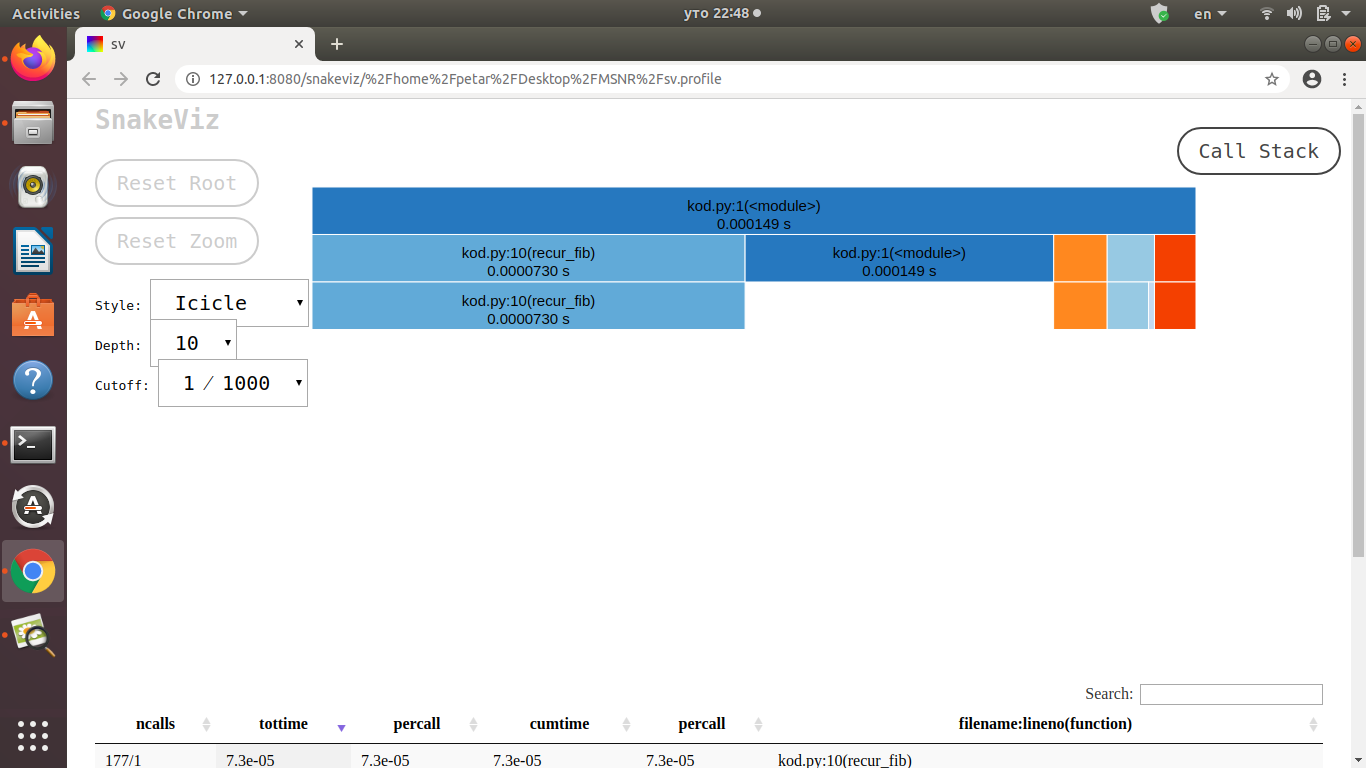
\includegraphics[trim={10cm 15cm 5cm 6.5cm},clip,scale=0.35]{MVJ_02_ProfajleriZaPython_ZecevicSmiljanicMilovanovicPopov/snakeviz1.png}
\end{center}
\caption{SnakeViz vizualizacija.}
\label{fig:snake_viz_1}
\end{figure}
Pored toga, SnakeViz za svaku funkciju može da prikaže vreme izvršavanja funkcije (u milisekundama i procentima), kao i liniju na kojoj se funkcija nalazi u kodu. Primer ovih statistika za funkciju koja računa rekurentno n-ti Fibonačijev broj dat je na slici \ref{fig:snake_viz_2}.
\begin{figure}[h!]
\begin{center}
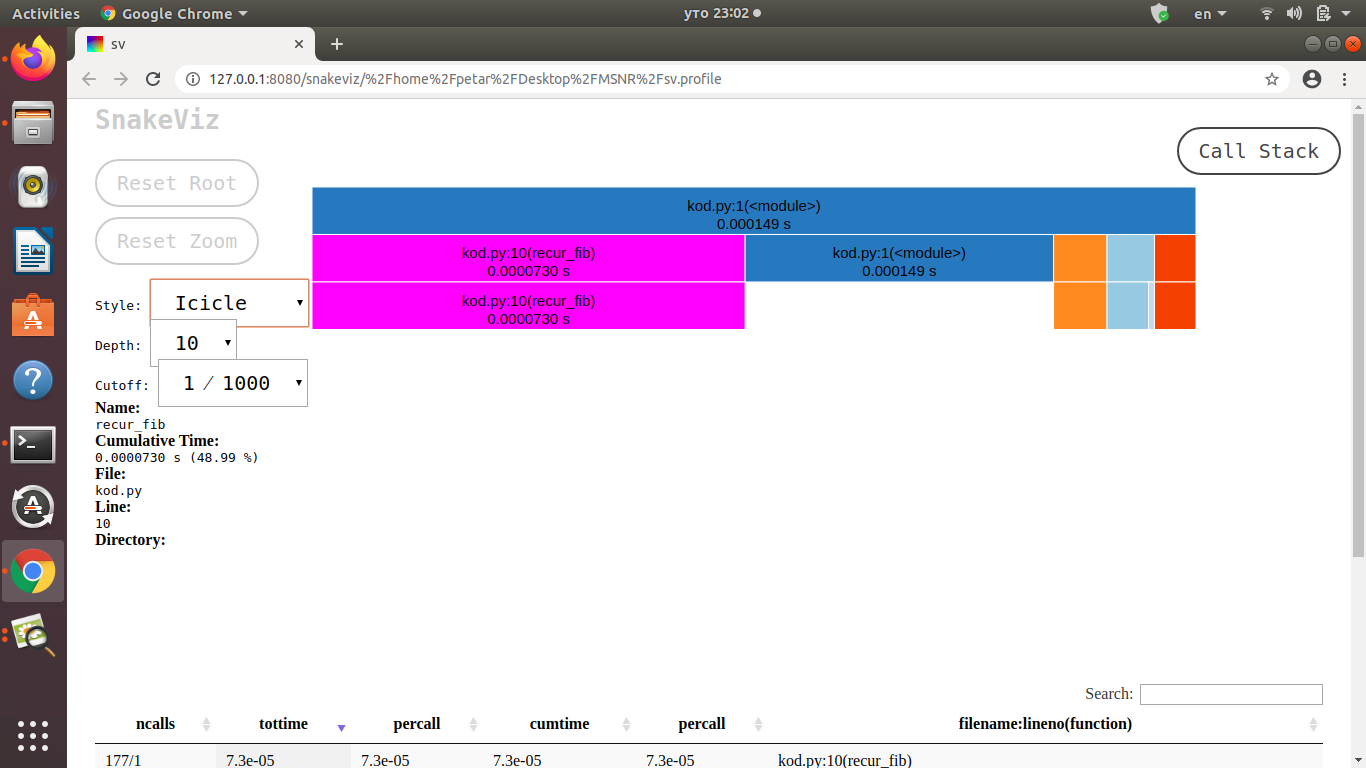
\includegraphics[trim={3cm 7.5cm 35cm 14cm},clip,scale=0.55]{MVJ_02_ProfajleriZaPython_ZecevicSmiljanicMilovanovicPopov/snakeviz2.png}
\end{center}
\caption{SnakeViz statistike.}
\label{fig:snake_viz_2}
\end{figure}
    
\subsection{Pycallgraph}
\label{profajler_4}
\textbf{Pycallgraph} je Python modul pomoću kog se na osnovu koda može dobiti graf poziva. Postoji podrška za Python 2.7+ i Python 3.3+ \cite{Pycallgraph}.
Moguće ga je pokrenuti iz komandne linije ili uključiti u kod.
Pycallgraph se instalira izvršavanjem sledeće komande:
\begin{lstlisting}[language=bash, belowskip=-\baselineskip]
  $ pip install pycallgraph
\end{lstlisting}
Osim toga, neophodno je imati instaliran {\em Graphviz} ili {\em Gephi} kako bi vizualizacija bila moguća:
\begin{lstlisting}[language=bash, belowskip=-\baselineskip]
  $ sudo apt-get install graphviz
\end{lstlisting}
Graf poziva se dobija u direktorijumu iz kog se pokreće naredna komanda:
\begin{lstlisting}[language=bash,frame=single, label=lst:pycallgraph, belowskip=-\baselineskip]
  $ pycallgraph graphviz -- ./test.py 
\end{lstlisting}
Format u kom se čuva izlaz se može jednostavno zadati korišćenjem opcije -f, a ukoliko se format ne zada podrazumevani će biti .png (pycallgraph.png). 
Detaljnije informacije o instalaciji i pokretanju alata mogu se naći na \cite{Pycallgraph}.
\subsubsection{Karakteristike alata}
Pri korišćenju ovog alata moguće je čvorove grafa poziva obojiti različitim bojama, u zavisnosti od toga koliko puta je funkcija pozvana, ili koliko je vremena ili memorije potrebno za njeno izvršavanje. Pored toga, različiti moduli programa mogu biti vizuelno grupisani kako bi graf bio lakši za razumevanje. Poslednja verzija ovog alata izašla je 2013. godine, ali i dalje se bez problema može koristiti \cite{Pycallgraph}.

\subsubsection{Primer primene}
Pokretanjem naredne komande nad test kodom \ref{lst:test_code}, sa opcijom {\em max-depth} pomoću koje se zadaje maksimalna dubina, dobijena je slika \ref{fig:pycallgraph4_1}.
\begin{lstlisting}[language=bash,frame=single, belowskip=-\baselineskip, label=lst:pycallgraph4_1]
  $ pycallgraph --max-depth=4  graphviz -- ./test.py
\end{lstlisting}
\begin{figure}[h!]
\begin{center}
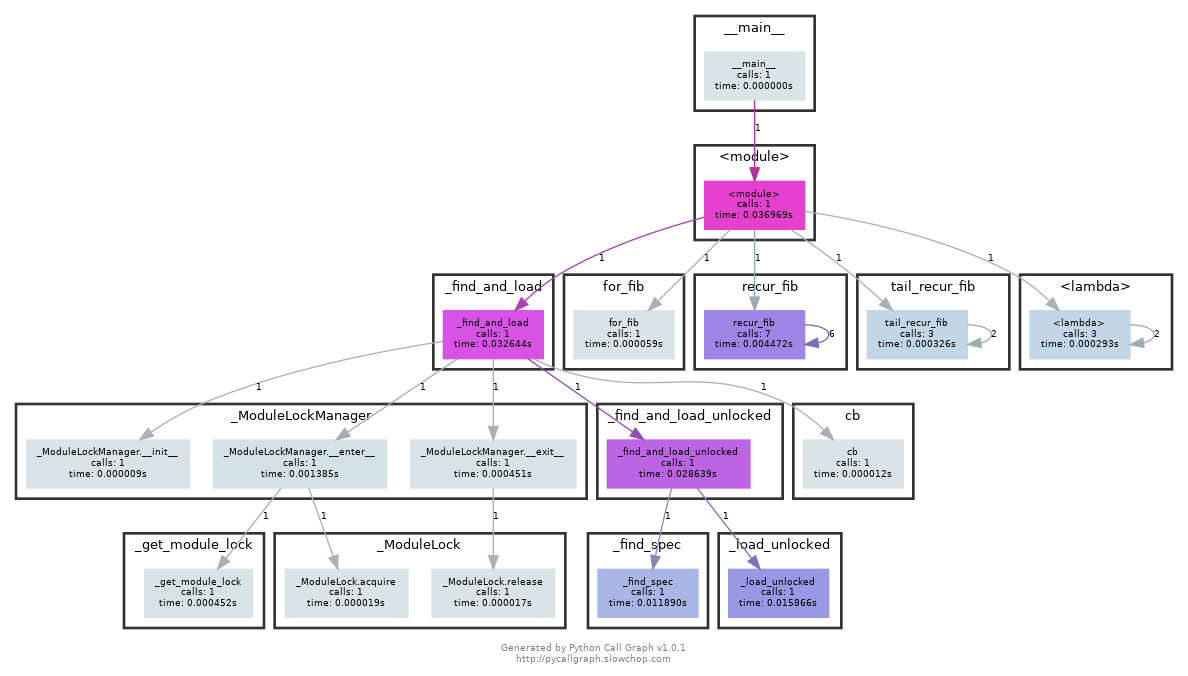
\includegraphics[scale=0.26]{MVJ_02_ProfajleriZaPython_ZecevicSmiljanicMilovanovicPopov/pycallgraph_depth4.png}
 \end{center}
 \caption{Pycallgraph vizualizacija za graf dubine 4.}
 \label{fig:pycallgraph4_1}
 \end{figure}
 Na slici \ref{fig:pycallgraph4_1} bojenje čvorova izvršeno je na osnovu vremena potrebnog za izvršavanje funkcija i broja poziva. To znači da su tamnijim bojama predstavljene funkcije koje su vremenski zahtevnije.
    
\subsection{Gprof2dot}
\label{profajler_5}
\textbf{Gprof2dot} je alat za vizualizaciju izlaza različitih profajlera u obliku grafa sa čvorovima. Napisan je u programskom jeziku Python. Rad je omogućen na bilo kojoj platformi na kojoj su instalirani Python i Graphviz. Komanda za instalaciju gprof2dot alata je:
\begin{lstlisting}[language=bash, belowskip=-\baselineskip] 
  $ pip install gprof2dot
\end{lstlisting}
Da bi se gprof2dot koristio, mora se generisati izlaz koji on može da čita. To se postiže narednom komandom:
\begin{lstlisting}[language=bash, belowskip=-\baselineskip]
  $ python3 -m cProfile -o output.pstats path/to/your/script arg1 arg2
\end{lstlisting}
Nakon toga potrebno je pokrenuti komandu za izvršavanje gprof2dot alata i čuvanje rezultata u obliku slike output.png:
\begin{lstlisting}[language=bash, frame=single, label=lst:gprof2dot, belowskip=-\baselineskip]
  $ gprof2dot.py -f pstats output.pstats | dot -Tpng -o output.png
\end{lstlisting}
\subsubsection{Karakteristike alata}
Korišćenjem dodatne opcije pri zadavanju komande za izvršavanje gprof2dot alata moguće je dobiti potkresano drvo, do čega se dolazi eliminacijom svih čvorova ispod zadatog limita. Jedna od prednosti ovog alata je to što korišćenjem boja uspeva da skrene pažnju na kritične delove koda. Neki od profajlera čiji izlaz gprof2dot može da čita su: Linux Perf, Valgrind's Callgrind Tool, Python Profilers, gprof, itd. \cite{gprof}. Pomoću njega funkcijski pozivi se mogu predstaviti u vidu grafa, što je korisno kada su programi veliki. Nekada je teško uočiti grešku gledajući sirove podatke, dok graf može značajno olakšati uočavanje istih. 
\subsubsection{Primer primene}
Komandom iznad (\ref{lst:gprof2dot}) poziva se gprof2dot, čime se generiše slika grafa i čuva u .png formatu. Primer je pokrenut za 30. Fibonačijev broj.

\begin{figure}[h!]
\begin{center}
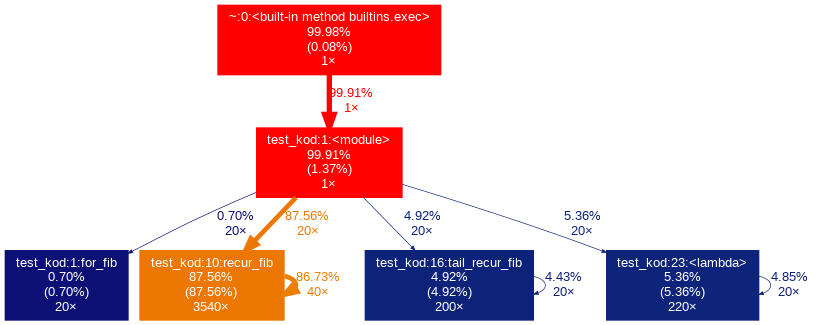
\includegraphics[scale=0.4]{MVJ_02_ProfajleriZaPython_ZecevicSmiljanicMilovanovicPopov/gprof2dot.png}
\end{center}
\caption{gprof2dot vizualizacija.}
\label{fig:gprof2dot_1}
\end{figure}
\begin{center}
\newpage
 Sadržaj jednog čvora: \newline
+---------------------------------------------+ \newline
|\hspace{32pt} ime funkcije\hspace{32.4pt}| \newline
| ukupno vreme\% ( vreme\%) | \newline
|\hspace{34pt} broj poziva\hspace{34.5pt}| \newline
+---------------------------------------------+\newline
\end{center}
gde je:
\begin{itemize}
\item ime funkcije - funkcija na koju se odnosi sadržaj čvora
\item ukupno vreme\% - odnosi se na procenat vremena provedenog u funkciji, u odnosu na ukupno vreme rada programa
\item vreme\% - odnosi se na procenat vremena provedenog u samo ovoj funkciji (bez poziva drugih funkcija)
\item broj poziva - koliko puta je funkcija pozvana (uključujući i rekruziju)
\end{itemize} 
Jedna grana grafa predstavlja poziv između funkcija. Ona povezuje roditeljsku i dete funkciju, gde je roditeljska funkcija ona koja poziva, dok je dete funkcija ona koja je pozvana iz roditeljske funkcije. Grana nosi informacije o tome koliko puta je roditelj pozvao dete funkciju, kao i procenat ukupnog vremena koje je potrebno da se izvršavanje prebaci sa jedne funkcije na drugu.

Sa slike \ref{fig:gprof2dot_1} može se videti da je najmanje vremena utrošeno na funkciju for\_fib, koja je pozivana najmanji broj puta (zato je plave boje). Funkcija recur\_fib oduzela je najviše vremena i pozivana je najviše puta (zato je narandžaste boje). Dva roditeljska čvora su crvene boje jer oni predstavljaju glavnu nit, koja traje koliko i ceo proces (zato i ima najveći procenat utrošenog vremena i samo jedan poziv). 

\subsection{Vprof}
\label{profajler_6}
	
\textbf{Vprof} radi tako što pokreće program, izvršava merenje i potom startuje lokalni server gde prikazuje rezultate u podrazumevanom veb pretraživaču. \\
Komanda za instalaciju alata je:
\begin{lstlisting}[language=bash, belowskip=-\baselineskip]
  $ pip install vprof
\end{lstlisting}
Pokretanje vprof alata izgleda ovako:
\begin{lstlisting}[language=bash, belowskip=-\baselineskip]
  $ vprof -c <config> <src>
\end{lstlisting}
Argument <config> podrazumeva sledeće opcije:
\begin{itemize}
    \item  p - profajler
    \item  m - graf memorije
    \item  h - toplotna mapa koda
    \item  c - CPU flejm graf
\end{itemize}

Prednost u odnosu na ostale alate ogleda se u tome što se rezultati prikazuju u interaktivnoj veb aplikaciji. Loša strana je to što se nalazi u konstantnom razvoju, pa može doći do bagova. Pokretanje vprof alata, prilikom kog se dobija vizualizacija izvršavanja koda u veb pretraživaču, realizuje se komandom:
\begin{lstlisting}[language=bash, belowskip=-\baselineskip]
  $ vprof -c p test_kod.py
\end{lstlisting}
\begin{figure}[h!]
\begin{center}
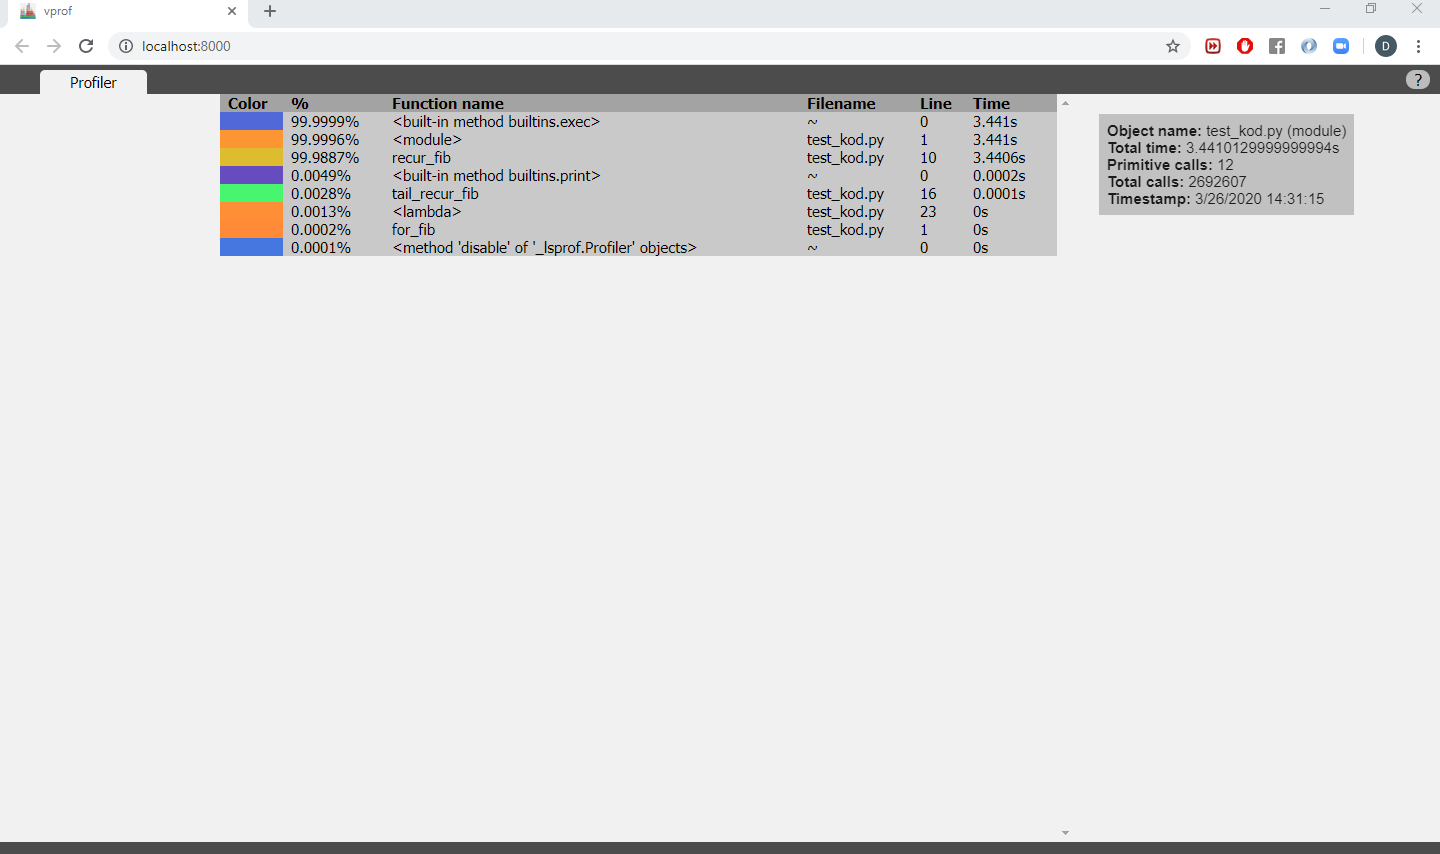
\includegraphics[trim={0cm 20cm 0cm 0cm},clip,scale=0.23]{MVJ_02_ProfajleriZaPython_ZecevicSmiljanicMilovanovicPopov/vprof.png}
\end{center}
\caption{vprof vizualizacija.}
\label{fig:vprof_1}
\end{figure}Detaljnije informacije o instalaciji i pokretanju alata mogu se naći na \cite{vprof}.
\section{Zaključak}
\label{sec:zaključak}
Kroz ovaj rad predstavljene su osnovne ideje procesa profajliranja. Čitalac je upoznat sa modulima za profajliranje u jeziku Python, kao i sa alatima za vizualizovanje statističkih izveštaja koje profajleri generišu. Korišćenjem alata \textbf{Py-Spy} predstavljeno je kako rade statistički profajleri i zašto su oni bitni, dok su kroz alate \textbf{SnakeViz}, \textbf{Pycallgraph}, \textbf{Gprof2dot} i \textbf{Vprof} predstavljene neke od mogućnosti determinističkih profajlera. Za sve alate prikazan je i ukratko objašnjen izlaz koji oni generišu kada se pokrenu nad test kodom \ref{lst:test_code}.

Prednost korišćenja profajlera je mogućnost dobijanja bolje slike o tome odakle je koja funkcija pozvana, koliko je njeno izvršavanje trajalo, da li je ona pozivala još neke funkcije, itd. Praćenjem toka izvršavanja programa mogu se uočiti razni propusti u kodu ili delovi koje je moguće optimizovati zbog toga što oduzimaju puno vremena. Dakle, kada razvoj softvera dođe u fazu da je potrebno debagovanje ili njegova optimizacija, profajliranje je nešto što značajno može ubrzati proces detekcije kritičnih delova. 

Čitalac se upućuje da nakon upoznavanja sa ovde predstavljenim alatima i njihovim osnovnim funkcionalnostima, samostalno istraži 
alate koji su mu se posebno dopali, korišćenjem referenci datih u poglavlju alata. Osim toga, dva dodatna modula za Python koja mogu biti interesantna za dalje istraživanje su: \textbf{line\_profiler} i \textbf{memory\_profiler}. Više o njima se može pročitati u poglavlju {\em IPython: Beyond Normal Python - Profiling and Timing Code} knjige \cite{vanderplas2016python}. Prvi modul omogućava linijsko profajliranje, dok drugi modul prati memorijsko opterećenje funkcija iz koda, za koje nije bilo prostora u ovom radu.  

\addcontentsline{toc}{section}{Literatura}
\appendix
\bibliography{seminarski} 
\bibliographystyle{plain}
\newpage
\appendix
\section{Dodatak}
\label{sec:dodatak}

\begin{lstlisting}[caption={Kod korišćen za testiranje modula i alata.},frame=single, label=lst:test_code]
# This program is used for testing purposes
def for_fib(n):
    a = 0
    b = 1
    for i in range(0, n):
        temp = a
        a = b
        b = temp + b
    return a

def recur_fib(n):
   if n <= 1:
       return n
   else:
       return(recur_fib(n-1) + recur_fib(n-2))
   
def tail_recur_fib(n, a = 0, b = 1): 
    if n == 0: 
        return a 
    if n == 1: 
        return b 
    return tail_recur_fib(n - 1, b, a + b)

functional_fib = (lambda x, a=1, b=0:
         b if x == 0
         else functional_fib(x - 1, a + b, a))

number = 10

print('Input number is: ' + str(number))
print('For loop Fibonacci ' + str(for_fib(number)))
print('Recursion Fibonacci: ' + str(recur_fib(number)))
print('Tail recursion Fibonacci: ' + str(tail_recur_fib(number)))
print('Functional Fibonacci: ' + str(functional_fib(number)))
\end{lstlisting}

\begin{lstlisting}[caption={Kod korišćen za testiranje modula cProfile i pstats.},frame=single, label=lst:cprofile_pstats, ]
import cProfile
import pstats
import io

number = 20
print('Input number is: ' + str(number))

def test_function():
    for i in range(0, 1000):
        for_fib(number)
        recur_fib(number)
        tail_recur_fib(number)
        functional_fib(number)

if __name__ == '__main__':
    prof = cProfile.Profile()
    prof.enable()
    # cProfile.run('test_function()', './izvestaj')
    test_function()
    prof.disable()

    s = io.StringIO()
    sortby = 'tottime'
    ps = pstats.Stats(prof, stream=s).sort_stats(sortby)
    ps.print_stats()
    print(s.getvalue())
\end{lstlisting}

\newpage

\begin{lstlisting}[caption={Primer profajliranja korišćenjem modula {\em time}.}, frame=single, label=lst:kod_time]
import time
# ocitamo vreme na pocetku
tic = time.time()
n = 5
print("Ja sada spavam {} sekundi.".format(n))
time.sleep(n)
# ocitamo vreme na kraju
toc = time.time()
print("Ukupno je proteklo {} sekundi.".format(toc-tic))
\end{lstlisting}

\begin{table}[h!]
 \begin{center}
 \label{table:performance}
 \scalebox{0.87}{
 \begin{tabular}{||l l l l||}
 \hline
  & Procesor & RAM & OS  \\ [0.5ex] 
 \hline\hline
 A - Anđelka & Intel Core i5-7360U @ 2.3GHz x 2 & 16GB & macOS Catalina \\
 \hline
 D - David & Intel Core i5-3210M @ 2.5Ghz x 2 & 8GB & Windows 10 \\
 \hline
 J - Jelisaveta & Intel Core i5-520M @ 2.4GHz x 4 & 6GB & Ubuntu 19.04 \\ 
 \hline
 P - Petar & Intel Core i3-6100U @ 2.3GHz x 4 & 4GB & Ubuntu 18.04 \\
 \hline
\end{tabular}}
\end{center}
\caption{Karakteristike računara.}
\end{table}

\end{document}